
%%%%%%%%%%%%%%%%%%%%%%%%%%%%%%%%%%% SETUP
\documentclass{classes/beamer_GeomaticaUA}
%\documentclass[handout]{Classes/beamer_GeomaticaUA}
\usepackage{styles/beamer_GeomaticaUA}
%\usepackage{styles/Amsterdam}
\usepackage{listings}
\renewcommand{\lstlistlistingname}{Codes}
\renewcommand{\lstlistingname}{Code}


%% LISTING ENVIRONMENTS-----------------------
% Java/c#
\lstnewenvironment{Java}{\lstset{
language=Java,                % choose the language of the code
 frame=Ltbr,
 framerule=0.2pt,
 aboveskip=0.5cm,
 framextopmargin=3pt,
 framexbottommargin=3pt,
 framexleftmargin=0.4cm,
 framesep=0.4pt,
 rulesep=0.4pt,
 %backgroundcolor=\color{white},
 rulesepcolor=\color{gray},
 stringstyle=\ttfamily\color{purple},
 showstringspaces = false,
 %basicstyle=\small\ttfamily,
 commentstyle=\color[rgb]{0.133,0.545,0.133},
 keywordstyle=\color[rgb]{0,0,1},%\bfseries 
 %morekeywords={text,serial,with,owner,to, replace, function, for, if, begin, loop, exit,
 %return,returns,cost,row,volatile,into, setof, double, precision,declare,record,reverse,boolean},
 numbers=left,
 numbersep=14pt,
 breaklines=true
}}{}

% SQL
\lstnewenvironment{SQL}{\lstset{
language=SQL,                % choose the language of the code
 frame=Ltbr,
 framerule=0.2pt,
 aboveskip=0.25cm,
 framextopmargin=3pt,
 framexbottommargin=3pt,
 framexleftmargin=0.4cm,
 framesep=0.4pt,
 rulesep=0.4pt,
 backgroundcolor=\color{white},
 rulesepcolor=\color{gray},
 stringstyle=\ttfamily\color{purple},
 showstringspaces = false,
 basicstyle=\tiny\ttfamily,
 commentstyle=\color[rgb]{0.133,0.545,0.133},
 keywordstyle=\color[rgb]{0,0,1},%\bfseries 
 morekeywords={text,serial,with,owner,to, replace, function, for, if, begin, loop, exit,
 return,returns,cost,row,volatile,into, setof, double, precision,declare,record,reverse,boolean},
 numbers=left,
 numbersep=14pt,
 breaklines=true,
 extendedchars=true,
 literate={á}{{\'a}}1 {é}{{\'e}}1 {í}{{\'i}}1 {ó}{{\'o}}1 {ú}{{\'u}}1 {ñ}{{\~n}}1 {¿}{{?`}}1
}}{}


% Defino un entorno CommandLine Linux
\lstnewenvironment{bash}{\lstset{
language=bash,                % choose the language of the code
 frame=Ltbr,
 framerule=0.2pt,
 aboveskip=0.25cm,
 framextopmargin=3pt,
 framexbottommargin=3pt,
 framexleftmargin=0.4cm,
 framesep=0.4pt,
 rulesep=0.4pt,
 backgroundcolor=\color{white},
 rulesepcolor=\color{gray},
 stringstyle=\ttfamily\color{purple},
 showstringspaces = false,
 basicstyle=\tiny\ttfamily,
 commentstyle=\color[rgb]{0.133,0.545,0.133},
 keywordstyle=\color[rgb]{0,0,1},%\bfseries
 morekeywords={cd,mkdir}
 numbers=left,
 numbersep=14pt,
 breaklines=true,
 extendedchars=true,
 literate={á}{{\'a}}1 {é}{{\'e}}1 {í}{{\'i}}1 {ó}{{\'o}}1 {ú}{{\'u}}1 {ñ}{{\~n}}1 {¿}{{?`}}1
}}{}


% PLR
\lstnewenvironment{PLR}{\lstset{
language=R,                % choose the language of the code
 frame=Ltbr,
 framerule=0.2pt,
 aboveskip=0.5cm,
 framextopmargin=3pt,
 framexbottommargin=3pt,
 framexleftmargin=0.4cm,
 framesep=0.4pt,
 rulesep=0.4pt,
 %backgroundcolor=\color{white},
 rulesepcolor=\color{gray},
 stringstyle=\ttfamily\color{purple},
 showstringspaces = false,
 %basicstyle=\small\ttfamily,
 commentstyle=\color[rgb]{0.133,0.545,0.133},
 keywordstyle=\color[rgb]{0,0,1},%\bfseries 
 morekeywords={text,serial,with,owner,to, replace, function, for, if, begin, loop, exit,
 return,returns,cost,row,volatile,into, setof, double, precision,declare,record,reverse},
 numbers=left,
 numbersep=14pt,
 breaklines=true
}}{}

% R
\lstnewenvironment{R}{\lstset{
language=R,                % choose the language of the code
 frame=Ltbr,
 framerule=0.2pt,
 aboveskip=0.5cm,
 framextopmargin=3pt,
 framexbottommargin=3pt,
 framexleftmargin=0.4cm,
 framesep=0.4pt,
 rulesep=0.4pt,
 %backgroundcolor=\color{white},
 rulesepcolor=\color{gray},
 stringstyle=\ttfamily\color{purple},
 showstringspaces = false,
 alsoother={:_\$},
 %basicstyle=\small\ttfamily,
 commentstyle=\color[rgb]{0.133,0.545,0.133},
 keywordstyle=\color[rgb]{0,0,1},%\bfseries 
 %morekeywords={text,serial,with,owner,to, replace, function, for, if, begin, loop, exit,
 %return,returns,cost,row,volatile,into, setof, double, precision,declare,record,reverse},
 numbers=left,
 numbersep=14pt,
 breaklines=true
}}{}

% PHP
\lstnewenvironment{PHP}{\lstset{
language=PHP,                % choose the language of the code
 frame=Ltbr,
 framerule=0.2pt,
 aboveskip=0.5cm,
 framextopmargin=3pt,
 framexbottommargin=3pt,
 framexleftmargin=0.4cm,
 framesep=0.4pt,
 rulesep=0.4pt,
 %backgroundcolor=\color{white},
 rulesepcolor=\color{gray},
 stringstyle=\ttfamily\color{purple},
 showstringspaces = false,
 %basicstyle=\small\ttfamily,
 commentstyle=\color[rgb]{0.133,0.545,0.133},
 keywordstyle=\color[rgb]{0,0,1},%\bfseries 
 numbers=left,
 numbersep=14pt,
 breaklines=true
}}{}

% Diagramas entidad relación
% Ver ejemplo en http://heisenbugs.blogspot.com.es/2010/10/making-great-er-diagrams-without.html
\usepackage{styles/tikz-er2}
\usetikzlibrary{positioning}
\usetikzlibrary{shadows}
\usetikzlibrary{mindmap}
% Diagramas UML
% Ver http://perso.ensta-paristech.fr/~kielbasi/tikzuml/index.php?lang=en
\usepackage{styles/tikz-uml}

%% ER styles
\tikzstyle{every entity} = [top color=white, bottom color=blue!30,
draw=blue!50!black!100, drop shadow]
\tikzstyle{every weak entity} = [drop shadow={shadow xshift=.7ex,
shadow yshift=-.7ex}]
\tikzstyle{every attribute} = [top color=white, bottom color=yellow!20,
draw=yellow, node distance=7em, drop shadow]
\tikzstyle{every relationship} = [top color=white, bottom color=red!20,
draw=red!50!black!100, drop shadow]
\tikzstyle{every isa} = [top color=white, bottom color=green!20,
draw=green!50!black!100, drop shadow]


%% Árboles de directorios
%\usepackage{tikz}
%\usetikzlibrary{trees}

%\tikzstyle{every node}=[draw=black,thick,anchor=west]
%\tikzstyle{selected}=[draw=red,fill=red!30]
%\tikzstyle{optional}=[dashed,fill=gray!50]

%%%%%%%%%%%%%%%%%%%%%%%%%%%%%%%%%%%
%\begin{frame}{Modelo Jerárquico}
%\begin{columns}
%\begin{column}{0.5\textwidth}
%\begin{center}

%\begin{tikzpicture}[%
%  grow via three points={one child at (0.5,-0.7) and
%  two children at (0.5,-0.7) and (0.5,-1.4)},
%  edge from parent path={(\tikzparentnode.south) |- (\tikzchildnode.west)}]
%  \node {País}
%    child { node {Prov A}}		
%    child { node [selected] {Prov C}
%      child { node {Muni C1}}
%      child { node [selected]{Muni C2}
%      	child { node [selected] {Parc 1}}
%      	child { node [selected] {Parc2}}
%      	child { node [selected] {Parc n}}
%      }
%      child [missing] {}	
%      child [missing] {}				
%	  child [missing] {}	
%      child { node [optional] {Muni C$n$}}
%    }
%    child [missing] {}				
%    child [missing] {}	
%    child [missing] {}				
%    child [missing] {}	
%    child [missing] {}							
%    child [missing] {}				
%    child { node [optional] {Prov $n$}};
%\end{tikzpicture}
%\end{center}
%\end{column}
%
%\begin{column}{0.5\textwidth}
%El modelo jerárquico organiza los datos en una estructura ramificada (\textit{tree structure}).\\[3ex]
%
%\textbf{Consulta:}\\
%Cultivos/superficie en el municipio C2\\[3ex]
%
%\textbf{Coste:} \\
%Una búsqueda por Prov, otra por Muni de la Prov C y calculamos las estadísticas para todos. No hay que seguir buscando.
%\end{column}
%\end{columns}
%\end{frame}

%%%%%%%%%%%%%%%%%%%%%%%%%%%%%%%%%%% METADATA
\author{Benito Zaragozí}
\title{Introducción al diseño de bases de datos espaciales}
\titlegraphic{
\includegraphics[height=0.6cm]{logos/logo_ua.png} \hspace{1cm} 
\includegraphics[height=1cm]{logos/iig}} 
\institute[GeomaticaLab]{Instituto Interuniversitario de Geografía\\Laboratorio de Geomática} 
\date{13 de noviembre de 2014}
\subject{Primera sesión del curso ``Diseño, creación y gestión de Bases de Datos Geográficas con PostGIS''}


%%%%%%%%%%%%%%%%%%%%%%%%%%%%%%%%%%% SLIDES
\begin{document}

\begin{frame}
\titlepage
\end{frame}

\section[Introducción]{Presentación y comentarios sobre la estructura del curso}
\subsection{Un poco de teoría y un montón de práctica}
\begin{frame}{¿Que vamos a hacer hoy?}
\begin{enumerate}
\item Programa del curso
\item ¿Qué es una geodatabase?
\item Caso práctico
\item Teoría y conceptos básicos
\item Diseño de un modelo de datos
\item Implementación en PostGIS
\end{enumerate}
\end{frame}

%%%%%%%%%%%%%%%%%%%%%%%%%%%%%%%%%%%
\begin{frame}{¿Qué es una geodatabase?}
\begin{block}{Definición de geodatabase}
Una geodatabase es una base de datos con tipos especiales para los objetos geométricos. Permite almacenar datos geométricos y proporciona funciones especiales, índices espaciales y lenguajes de consulta (SQL). Una base de datos espacial es a menudo utilizado como un simple contenedor de almacenamiento para los datos espaciales, pero puede ser mucho más que eso.
\end{block}

\begin{exampleblock}{Geodatabases relacionales}
\begin{itemize}
\item \underline{Comerciales:} \href{http://en.wikipedia.org/wiki/Oracle\_Spatial}{Oracle Spatial}, SQL Server (2008), IBM DB2 Spatial, IBM Informix Spatial, MapInfo SpatialWare y \href{http://help.arcgis.com/es/arcgisserver/10.0/help/arcgis\_server\_dotnet\_help/index.html\#//009300000115000000}{ESRI ArcSDE}.
\item \underline{Libres:} MySQL Spatial, \href{http://en.wikipedia.org/wiki/SpatiaLite}{SpatiaLite} y PostGIS.
\end{itemize}
\end{exampleblock}
\end{frame}

%%%%%%%%%%%%%%%%%%%%%%%%%%%%%%%%%%%
\begin{frame}{Otras geodatabases alternativas (NoSQL)}
\begin{block}{Definición de NoSQL}
Según \href{http://nosql-database.org/}{nosql-database.org}, es la nueva generación de bases de datos que se distinguen por las siguientes características:
\begin{itemize}
\item No-relacionales.
\item Distribuidas.
\item Open-source
\item Horizontalmente escalables.
\end{itemize}
\end{block}

\begin{block}{NoSQL con componente espacial}
\begin{itemize}
\item Perst, \href{http://paralleluniverse.co/product/}{SpaceBase} y ¿DB4O-spatial? 
\item Neo4j y AllegroGraph.
\item MongoDB y CouchDB.
\item \href{http://cartodb.com/}{CartoDB} y StormDB.
\end{itemize}
\end{block}
\end{frame}

%%%%%%%%%%%%%%%%%%%%%%%%%%%%%%%%%%%
\begin{frame}{SGBD espaciales vs SIG orientados a la aplicación}
La relación entre SIG y Sistemas Gestores de Bases de Datos (SGBD) es cada vez más cercana y está tomando un interés creciente. Existen varios motivos que explican dicho interés:

\begin{columns}
\begin{column}{0.5\textwidth}
\begin{exampleblock}{Ventajas}
\begin{itemize}
\item Reducción de la redundancia de datos
\item Aumento de la integridad de datos
\item Independencia de datos
\item Seguridad de los datos
\item Mantenimiento eficiente
\item Visión Corporativa
\end{itemize}
\end{exampleblock}
\end{column}

\begin{column}{0.5\textwidth}
\begin{alertblock}{Inconvenientes}
\begin{itemize}
\item Costes más elevados
\item Personal adicional
\item Aumento del tiempo de desarrollo
\item Riesgo centralizado
\item Anonimato de los datos
\item Racionalidad excesiva
\end{itemize}
\end{alertblock}
\end{column}
\end{columns}
\end{frame}


\section[Conceptos]{Conceptos básicos en tecnologías de la información}
\subsection{De los hechos a la sabiduría}
%%%%%%%%%%%%%%%%%%%%%%%%%%%%%%%%%%%
\begin{frame}{El mundo real}

\begin{block}{hecho, cha. (RAE)}
(Del part. irreg. de hacer; lat. factus).
...
5. m. Cosa que sucede.
6. m. Asunto o materia de que se trata.
\end{block}

\begin{exampleblock}{Ejemplo lab: hechos}
``Actualmente, en el lab trabajan seis personas: Alfredo, José Manuel, José Tomás, Pepe, Miguel y Benito. Alfredo es el miembro del lab con mayor experiencia, tiene cincuenta ``tacos'', seguido de JM y JT, que ya no cumplen los cuarenta. A continuación, Miguel y Pepe tienen más de treinta y cinco, pero aún se les puede considerar jóvenes. Finalmente, por Benito parece que no pasa el tiempo, pero ya casi tiene la edad de Cristo al morir...''
\end{exampleblock}

\end{frame}

%%%%%%%%%%%%%%%%%%%%%%%%%%%%%%%%%%%
\begin{frame}{Datos}
Un dato es un hecho registrado en cualquier formato y que puede ser útil para un usuario. Se trata de información no procesada.

\begin{exampleblock}{Ejemplo lab: datos}
lab, Alfredo, 46, José Manuel,José Tomás, Pepe, Miguel, Benito, 50, JM, 33, JT, 49, 39, 36
\end{exampleblock}

Si no aportamos estructura ni contexto, los datos son difícilmente utilizables.

\end{frame}

%%%%%%%%%%%%%%%%%%%%%%%%%%%%%%%%%%%
\begin{frame}{Modelo Relacional}
El modelo E-R (entidad-relación) representa el ``mundo real'' como un conjunto de entidades y relaciones entre estos objetos (entidad, conjunto de entidades, atributos y relaciones). Es el primer modelo basado en una teoría preexistente, propuesta por E. F. Codd en 1970. \\[3ex]

Desde sus orígenes es el modelo más utilizado, pero su simplicidad ha provocado que se investiguen los modelos Orientados a Objetos y Objeto-relacional.
\end{frame}

%%%%%%%%%%%%%%%%%%%%%%%%%%%%%%%%%%%
\begin{frame}{Teoría del Modelo Relacional (I)}
El modelo relacional se estructura en tablas con las siguientes características básicas:
\begin{itemize}
\item Relación, tupla, atributos, grado, cardinalidad, clave primaria y dominio.
\item Columnas únicas (nombre y dominio)
\item Registros atómicos y únicos
\item Columnas y filas \alert{no guardan orden alguno}
\item Tabla (real) y vista (virtual)
\item Integridad de entidades (claves primarias) e integridad referencial (claves externas)
\end{itemize}
\end{frame}

%%%%%%%%%%%%%%%%%%%%%%%%%%%%%%%%%%%
\begin{frame}{Teoría del Modelo Relacional (II)}
\begin{center}
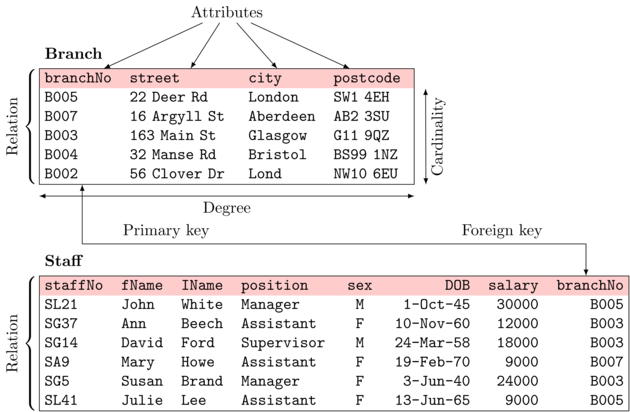
\includegraphics[width=0.8\textwidth]{images/relational_model.png} 
\end{center}
\end{frame}

%%%%%%%%%%%%%%%%%%%%%%%%%%%%%%%%%%%
\begin{frame}{Teoría del Modelo Relacional (III)}
El modelo relacional proporciona un conjunto de operadores para manipular las tablas (\href{http://es.wikipedia.org/wiki/\%C3\%81lgebra_relacional}{álgebra relacional}). Esto se verá en detalle en la sesión de SQL (\textit{Structured Query Language}).
\end{frame}

%%%%%%%%%%%%%%%%%%%%%%%%%%%%%%%%%%%
\begin{frame}{Bases de datos}
Una base de datos es una colección de datos interrelacionados. También son bases de datos:
\begin{itemize}
\item Una guía telefónica o una agenda
\item La programación de TV
\item Un sistema de reserva de billetes de autobús
\item Los ficheros almacenados en el disco duro de un PC
\end{itemize}

\begin{exampleblock}{Ejemplo lab: base de datos}
\begin{center}
\begin{tabular}{|c|c|c|}
\hline 
\textbf{Nombre} & \textbf{Edad} & \textbf{Alias} \\ 
\hline 
Alfredo & 49 & • \\ 
\hline 
José Manuel & 47 & JM \\ 
\hline 
José Tomás & 43 & JT \\ 
\hline 
Miguel & 39 & • \\ 
\hline 
Pepe & 36 & • \\ 
\hline 
Benito & 33 & • \\ 
\hline 
\end{tabular} 
\end{center}
\end{exampleblock}

\end{frame}

%%%%%%%%%%%%%%%%%%%%%%%%%%%%%%%%%%%
\begin{frame}{Sistema Gestor de Bases de Datos}
Un SGBD o DBMS proporciona el \textbf{software} necesario para organizar los datos de un modo flexible. Incluye herramientas para añadir, modificar o eliminar datos, realizar preguntas sobre los datos almacenados y producir informes de un modo rápido.

Para la elección del SGBD es muy recomendable tener en cuenta el Modelo de los Datos. Esto puede ahorrar mucho trabajo.
\end{frame}

%%%%%%%%%%%%%%%%%%%%%%%%%%%%%%%%%%%
\begin{frame}{Información}
Datos procesados, organizados y comunicados de un modo coherente. La información también puede ser vista como la respuesta a una pregunta.

\begin{exampleblock}{Ejemplo lab: información}
\begin{itemize}
\item Todos los miembros del Lab son mayores de 32 años
\item Ningún miembro del lab se jubilará en los próximos 5 años
\item Sólo los miembros cuyo nombre es ``José'' tienen un alias, a Pepe no le hace falta...
\item etc, etc
\end{itemize}
\end{exampleblock}

\end{frame}

%%%%%%%%%%%%%%%%%%%%%%%%%%%%%%%%%%%
\begin{frame}{Conocimiento}
Información analizada, extraída y evaluada con un propósito. Este nivel de comprensión permite participar en procesos de toma de decisiones.

\begin{exampleblock}{Ejemplo lab: conocimiento}
En el caso de que no cambie nada, en menos de 20 años la plantilla del laboratorio estará muy envejecida. Esto puede tener consecuencias en el mantenimiento de los servicios. Hemos decidido
\end{exampleblock}

\end{frame}

%%%%%%%%%%%%%%%%%%%%%%%%%%%%%%%%%%%
\begin{frame}{Sabiduría}
Una vez que los conocimientos obtenidos son aplicados, estos producen efectos (buenos, malos, etc). Este proceso produce nuevos datos e información, se trata de un conocimiento más útil para la solución de problemas.

\vspace{1cm}

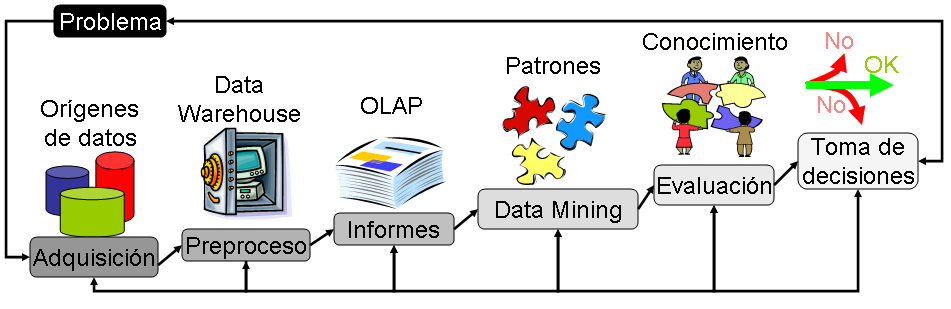
\includegraphics[width=\textwidth]{images/proceso_KDD_mio.png} 

\end{frame}

\section[Caso práctico]{Investigación previa y pasos a seguir}
\subsection{Gestión de espacios de una corporación}
%%%%%%%%%%%%%%%%%%%%%%%%%%%%%%%%%%%
\begin{frame}{Introducción}
\begin{block}{Problema}
La UA, con decenas de edificios y miles de empleados, quiere optimizar la gestión espacios. Los gerentes sospechan que el gasto en limpieza es desproporcionado en algunos departamentos. Además, entre otros diversos problemas, bromean sobre el rumor de que en los edificios próximos a la cafetería se hacen más horas extra. No obstante, no tienen un modo de analizar este tipo de situaciones. La información depende de distintos departamentos:
\begin{itemize}
\item Cartografía digital de los proyectos de cada edificio (Oficina técnica de proyectos).
\item Un código para denominar a cada estancia (Gestión de espacios docentes).
\item Un completo listado de personal (Gestión económica).
\end{itemize}
\end{block}
\end{frame}

%%%%%%%%%%%%%%%%%%%%%%%%%%%%%%%%%%%
\begin{frame}{Introducción II}
Una geodatabase es un medio ideal para solucionar estos y otros posibles problemas. Analizar los datos de un modo sistemático dependerá de que superemos con éxito una serie de fases.

\begin{block}{Objetivos específicos}
\begin{enumerate}
\item Definir un modelo de base de datos (ER, OO, Graph, etc).
\item Escoger un SGBD apropiado (centenares de usuarios).
\item Implementar la base de datos e incorporar toda la información disponible.
\item Desarrollar métodos para responder a las preguntas específicas de los gestores y del público en general.
\item Publicar los informes de un modo dinámico, para que los usuarios encuentren lo que necesitan con poco esfuerzo.
\end{enumerate}
\end{block}
\end{frame}


%%%%%%%%%%%%%%%%%%%%%%%%%%%%%%%%%%%
\begin{frame}{¿Por dónde empezamos?}
\begin{enumerate}
\item Conocer el problema de estudio (disciplina, conocimientos, experiencia, etc)
\item Análisis de necesidades (\href{http://es.wikipedia.org/wiki/Martillo_de_oro}{Martillo de Maslow})
\item Modelizar los datos (ER, UML, otros)
\item Seleccionar un SGBD (PostgreSQL, Oracle, MySQL, etc)
\item Implementar el modelo (\textit{Data Definition Language} -- SQL)
\item Mantenimiento y gestión (acualizaciones, backups, desarrollos, etc)
\end{enumerate}
\end{frame}

%%%%%%%%%%%%%%%%%%%%%%%%%%%%%%%%%%%
\begin{frame}{Análisis de necesidades}
El análisis de necesidades es específico de cada organización pero, como mínimo, debería responder unas preguntas básicas:

\begin{itemize}
\item ¿Cuantos registros almacenaremos y durante cuanto tiempo?
\item ¿Quien utilizará la base de datos y para qué?
\item ¿Los datos se modificarán? y, si es así, ¿con cuanta frecuencia?
\item ¿Quien mantendrá la BD?
\item ¿Qué hardware hay disponible?, ¿hay presupuesto para algo mejor?
\item ¿Quien será el responsable de los datos?
\item Los datos se consultarán on-line, ¿cuantas conexiones se realizarán?
\end{itemize}
\end{frame}


%%%%%%%%%%%%%%%%%%%%%%%%%%%%%%%%%%%
\begin{frame}{Diseño de bases de datos relacionales}
Dos aproximaciones principales:
\begin{enumerate}
\item  Diseño de arriba abajo (top-down design)
\begin{itemize}
\item Desarrollo de un modelo conceptual (p. ej. ER, UML, etc)
\item Reducción del modelo conceptual a relaciones
\item Uso de la normalización como técnica de validación del modelo (si el modelo está bien hecho no hará falta más normalización)
\end{itemize}

\item Diseño de abajo arriba (bottom-up design)
\begin{itemize}
\item Diseño por descomposición
\item Uso de normalización para crear las relaciones a partir de una tabla plana
\end{itemize}
\end{enumerate}
\end{frame}

\section[Modelo ER]{Modelo Entidad-Relación (ER)}
\subsection{Diagramas Entidad-Relación}
%%%%%%%%%%%%%%%%%%%%%%%%%%%%%%%%%%%
\begin{frame}{¿Qué es un modelo Entidad-Relación?}
En un modelo ER el ``mundo real'' es descrito como una colección de entidades interrelacionadas. Estos modelos son representaciones con una notación ``conocida'', la cual permite una mejor comunicación entre los miembros del equipo que diseñan la base de datos. El modelo ER existe desde 1976 y fue propuesto por P. \textbf{Chen}. A pesar de su extendido uso, nunca ha sido estandarizado, por lo que conviene recordar que existen distintas notaciones ER:

\begin{columns}
\begin{column}{0.5\textwidth}
\begin{itemize}
\item \textbf{Chen}
\item Crow's foot notation
\item UML class diagrams
\item Bachman notation
\item Barker's Notation
\end{itemize}
\end{column}

\begin{column}{0.5\textwidth}
\begin{itemize}
\item IDEF1X[13]
\item Martin notation
\item Merise
\item Object-Role Modeling
\end{itemize}
\end{column}
\end{columns}

\end{frame}

%%%%%%%%%%%%%%%%%%%%%%%%%%%%%%%%%%%
\begin{frame}{¿Qué es un diagrama ER?}

Un diagrama Entidad-Relación es una herramienta gráfica para modelizar datos. Un ER consiste en:
\begin{itemize}
\item Una colección de entidades definidas
\item Una colección de relaciones entre dichas entidades
\item Atributos asociados tanto a las entidades como a las relaciones 
\end{itemize}

En un diagrama ER las relaciones reciben un nombre. Otros aspectos de la relación suelen ir implícitos pero también pueden representarse si es necesario.

\bigskip
¡¡Ojo!! En la práctica nos referimos a entidades y relaciones, cuando en realidad se trata de definiciones de entidades y definiciones de relaciones. 
\end{frame}


%%%%%%%%%%%%%%%%%%%%%%%%%%%%%%%%%%%
\begin{frame}{Entidad con atributos}
\begin{center}
\resizebox{\textheight}{!}{%
%Requiere setup del package ER-tikz
\begin{tikzpicture}[node distance=7em]
\node[entity] (person) {Persona};
\node[attribute] (pid) [left of=person] {\key{ID}} edge (person);
\node[attribute] (name) [above left of=person] {Nombre} edge (person);
\node[multi attribute] (phone) [above of=person] {Teléfono} edge (person);
\node[attribute] (address) [above right of=person] {Dirección} edge (person);
\node[attribute] (street) [above right of=address] {Calle} edge (address);
\node[attribute] (city) [right of=address] {Ciudad} edge (address);
\node[derived attribute] (age) [right of=person] {Edad} edge (person);
\end{tikzpicture}
}
\end{center}
\end{frame}


%%%%%%%%%%%%%%%%%%%%%%%%%%%%%%%%%%%
\begin{frame}{Relaciones uno-a-uno}

\begin{center}
%Requiere setup del package ER-tikz
\begin{tikzpicture}[node distance=8em]
\node[entity] (person) {Persona};
\node[relationship] (uses) [right of=person] {Uses} edge [->] node[auto,swap] {N} (person);
\node[entity] (tool) [right of=uses] {Estancia} edge [<-] node[auto,swap] {N} (uses);
\end{tikzpicture}
\end{center}

\begin{itemize}
\item Cada persona está asociada como máximo a una estancia
\item Cada estancia está asociada como máximo a una persona
\end{itemize}

\end{frame}


%%%%%%%%%%%%%%%%%%%%%%%%%%%%%%%%%%%
\begin{frame}{Relaciones uno-a-muchos}

\begin{center}
%Requiere setup del package ER-tikz
\begin{tikzpicture}[node distance=8em]
\node[entity] (person) {Persona};
\node[relationship] (uses) [right of=person] {Uses}
edge [->] node[auto,swap] {1} (person);
\node[entity] (tool) [right of=uses] {Estancia}
edge node[auto,swap] {N} (uses);
\end{tikzpicture}
\end{center}
\begin{itemize}
\item Cada persona está asociada cero o más estancias
\item Cada estancia está asociada como máximo a una persona
\end{itemize}

\end{frame}

%%%%%%%%%%%%%%%%%%%%%%%%%%%%%%%%%%%
\begin{frame}{Relaciones muchos-a-muchos}

\begin{center}
%Requiere setup del package ER-tikz
\begin{tikzpicture}[node distance=8em]
\node[entity] (person) {Persona};
\node[relationship] (uses) [right of=person] {Uses}
edge node[auto,swap] {N} (person);
\node[entity] (tool) [right of=uses] {Estancia}
edge node[auto,swap] {M} (uses);
\end{tikzpicture}
\end{center}

\begin{itemize}
\item Cada persona está asociada cero o más estancias
\item Cada estancia está asociada con cero o más personas
\end{itemize}

\end{frame}

%%%%%%%%%%%%%%%%%%%%%%%%%%%%%%%%%%%
\begin{frame}{Relación uno-a-muchos, con participación total}
El nivel de participación es otro tipo de restricción en una relación. El nivel de participación puede ser:
\begin{itemize}
\item Parcial $\rightarrow$ Solamente algunas estancias están ocupadas por personas 
\item Total $\rightarrow$ Todas las personas usan por lo menos una estancia
\end{itemize}


\begin{center}
%Requiere setup del package ER-tikz
\begin{tikzpicture}[node distance=8em]
\node[entity] (person) {Persona};
\node[relationship] (uses) [right of=person] {Uses} edge [total] (person);
\node[entity] (tool) [right of=uses] {Estancia} edge (uses);
\end{tikzpicture}
\end{center}

\end{frame}

%%%%%%%%%%%%%%%%%%%%%%%%%%%%%%%%%%%
\begin{frame}{Relación muchos a muchos, con cardinalidad especificada}

\begin{center}
%Requiere setup del package ER-tikz
\begin{tikzpicture}[node distance=8em]
\node[entity] (person) {Persona};
\node[relationship] (uses) [right of=person] {Uses} edge node[auto,swap] {0..*} (person);
\node[entity] (tool) [right of=uses] {Estancia} edge node[auto,swap] {1..3} (uses);
\end{tikzpicture}
\end{center}

\begin{itemize}
\item Cada persona está asociada a una estancia como mínimo y tres como máximo
\item Cada estancia puede estar ocupada por entre cero y \textit{n} personas
\end{itemize}

\end{frame}

%%%%%%%%%%%%%%%%%%%%%%%%%%%%%%%%%%%
\begin{frame}{Relaciones con atributos}
En algunos casos, una relación necesita tener atributos. En este caso el ``periodo'' es el tiempo que dura la relación y afecta tanto a las personas como a la ocupación de la estancia.

\begin{center}
\resizebox{!}{0.25\textwidth}{%Requiere setup del package ER-tikz
\begin{tikzpicture}[node distance=8em]
\node[entity] (person) {Persona};
\node[attribute] (pid) [left of=person] {\key{ID}} edge (person);
\node[attribute] (name) [above left of=person] {Nombre} edge (person);

\node[relationship] (uses) [right of=person] {Uses} edge node[auto,swap] {N} (person);
\node[attribute] (timelapse) [above of=uses, node distance=6em] {periodo} edge (uses);

\node[entity] (room) [right of=uses] {Estancia} edge node[auto,swap] {M} (uses);
\node[attribute] (pid) [right of=room] {\key{ID}} edge (room);
\node[derived attribute] (area) [above right of=room] {Superficie} edge (room);
\end{tikzpicture}}
\end{center}

\begin{itemize}
\item Cada persona está asociada cero o más estancias
\item Cada estancia está asociada con cero o más personas
\end{itemize}

\end{frame}

%%%%%%%%%%%%%%%%%%%%%%%%%%%%%%%%%%%
\begin{frame}{Entidades débiles}
Las entidades débiles existen únicamente mientras están asociadas a otras entidades. Se caracterizan por:
\begin{itemize}
\item No tienen clave primaria
\item Contienten un conjunto de atributos que sirven para discriminarlas
\item Necesitan ser consideradas en conjunción con las entidades fuertes
\end{itemize}

\begin{center}
\resizebox{\textheight}{!}{%Requiere setup del package ER-tikz
\begin{tikzpicture}[node distance=8em]
\node[entity] (building) {Edificio};
\node[ident relationship] (has) [right of=building] {Has} edge [->] (building);
\node[weak entity] (room) [right of=has] {Estancia} edge [total] (has);
\node[attribute] (roomnum) [above of=room, node distance=6em]
{\discriminator{Código}} edge (room);
\end{tikzpicture}}
\end{center}

\end{frame}

%%%%%%%%%%%%%%%%%%%%%%%%%%%%%%%%%%%
\begin{frame}{Especialización/generalización}

\begin{center}
\resizebox{0.6\paperheight}{!}{%Requiere setup del package ER-tikz
\begin{tikzpicture}[node distance=7em]
\node[entity] (empleado) {Empleado};
\node[isa] (isa1) [below of=empleado,node distance=5em] {ISA}
edge node [auto,swap] {disjoint} (empleado);
\node [entity] (pdi) [below left of=isa1] {PDI} edge (isa1);
\node [entity] (pas) [below right of=isa1] {PAS} edge (isa1);
\node[isa] (isa2) [below of=pdi,node distance=5em] {ISA}
edge [total] (pdi);
\node [entity] (docente) [below left of=isa2] {Docente} edge (isa2);
\node [entity] (investigador) [below right of=isa2] {Investigador} edge (isa2);
\end{tikzpicture}}
\end{center}

\end{frame}

%%%%%%%%%%%%%%%%%%%%%%%%%%%%%%%%%%%
\begin{frame}{Agregación}

\begin{center}
\resizebox{0.8\textheight}{!}{%Requiere setup del package ER-tikz
\begin{tikzpicture}[node distance=7em]
\node[entity] (person) {Alumno};
\node[relationship] (uses) [right of=person] {Uses} edge (person);
\node[entity] (tool) [right of=uses] {PC} edge (uses);
\node[relationship] (watches) [below of=uses] {Watches} edge (uses);
\node[entity] (boss) [below of=watches] {Profesor} edge (watches);
\node[rectangle, draw=gray, fit=(person) (uses) (tool), inner sep=1em] {};
\end{tikzpicture}}
\end{center}

\end{frame}

%%%%%%%%%%%%%%%%%%%%%%%%%%%%%%%%%%%
\begin{frame}{Modelo ER básico de la UA}


\begin{center}
\resizebox{!}{0.6\textwidth}{%Requiere setup del package ER-tikz
\begin{tikzpicture}[node distance=8em]
\node[entity] (person) {Persona};
\node[attribute] (dni) [below of=person] {\key{DNI}} edge (person);
\node[attribute] (pname) [above left of=person] {Nombre} edge (person);
\node[attribute] (psurnames) [above of=person] {Apellidos} edge (person);
\node[derived attribute] (page) [below left of=person] {Edad} edge (person);
\node[attribute] (contrato) [left of=person, node distance=10em] {Contrato} edge (person);
\node[derived attribute] (extra) [above left of=contrato, node distance=6em] {Horas extra} edge (contrato);
\node[derived attribute] (holidays) [below left of=contrato, node distance=6em] {Vacaciones} edge (contrato);


\node[relationship] (works) [right of=person] {Trabaja} edge node[auto,swap] {N} (person);
\node[attribute] (timelapse) [above of=works, node distance=6em] {periodo} edge (works);



\node[entity] (room) [right of=works] {Estancia} edge node[auto,swap] {M} (works);
\node[attribute] (rid) [right of=room] {\key{Código}} edge (room);
\node[attribute] (use) [below right of=room] {Uso} edge (room);
\node[attribute] (rgeom) [above right of=room] {Geometry} edge (room);
\node[derived attribute] (rarea) [above right of=rgeom] {Superficie} edge (rgeom);
\node[derived attribute] (rdens) [above left of=rgeom] {Densidad} edge (rgeom);


\node[ident relationship] (has) [below of=works, node distance=12em] {Has} edge [->] (works);

\node[weak entity] (department) [below of=has, node distance=6em] {Departamento} edge [total] (has);
\node[attribute] (did) [right of=department] {\discriminator{ID}} edge (department);
\node[attribute] (dname) [left of=department] {Nombre} edge (department);


\node[rectangle, draw=gray, fit=(dni) (rarea) (extra), inner sep=1em] {};

\end{tikzpicture}}
\end{center}


\end{frame}

%%%%%%%%%%%%%%%%%%%%%%%%%%%%%%%%%%%
\begin{frame}{Normalización}

\end{frame}

\section[Implementación]{Implementación del modelo}
\subsection{Modelo relacional y SQL}
%%SQL entre otros lenguajes

%%%%%%%%%%%%%%%%%%%%%%%%%%%%%%%%%%%
\frame{\frametitle{Diagrama Entidad-Relación (físico)}
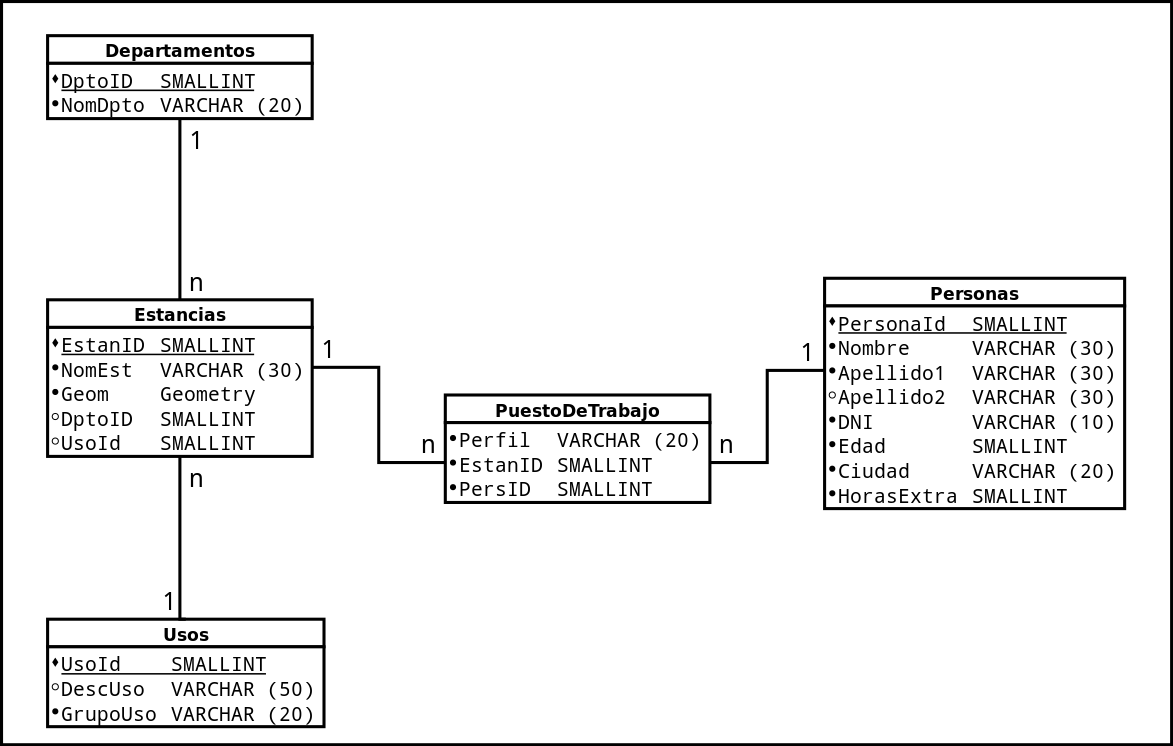
\includegraphics[width=\textwidth]{images/ER.png}
}

%%%%%%%%%%%%%%%%%%%%%%%%%%%%%%%%%%%
\begin{frame}[fragile]
\frametitle{Creación de una base de datos PostGIS}

\begin{block}{CREATE DATABASE y CREATE EXTENSION}
Desde el terminal invocamos \textbf{psql}, la consola interactiva de PostgreSQL, y nos conectamos con un usuario con privilegios para crear una base de datos. Una vez creada (\textit{CREATE DATABASE}), instalamos sobre ella la extensión \textbf{postgis} (\textit{CREATE EXTENSION}). 
\end{block}

\lstset{caption=Creación de la base de datos geográfica,label=bash:createDB}
\begin{bash}
psql -U user -h localhost -d postgres
CREATE DATABASE ua WITH ENCODING = 'UTF8';
\connect ua   ## Nos conectamos a la nueva base de datos
CREATE EXTENSION postgis;
\q            ## Cerramos la sesión psql
\end{bash}


\end{frame}

%%%%%%%%%%%%%%%%%%%%%%%%%%%%%%%%%%%
\begin{frame}[fragile]
\frametitle{Importación de estancias}

\begin{block}{shp2pgsql}
\setbeamerfont{footnote}{size=\tiny}
La utilidad \textbf{shp2pgsql} permite volcar \textit{shapefiles} en PostgreSQL como entidades PostGIS. Usaremos un \textit{snapshot} de las plantas bajas de los edificios del Campus de San Vicente\footnote[frame]{Fuente: \href{http://www.sigua.ua.es}{SIGUA}(Sistema de Información Geográfica de la UA)}.
\end{block}

\lstset{caption=Importación de estancias,label=bash:importarEstancias}
\begin{bash}
## Trabajamos en nuestro directorio de usuario
cd
## Descargamos archivo comrpimido con fichero shape de SIGUA
wget https://github.com/labgeo/postgis-intro/raw/2015edition/data/shapefiles/siguapb/siguapb.tar.lz
## Extraemos fichero shape en subdirectorio siguapb
mkdir siguapb; tar --lzip -xvf siguapb.tar.lz -C siguapb
## Importamos a PostgreSQL con la utilidad shp2pgsql
shp2pgsql -s 25830 siguapb/siguapb.shp public.estancias  | psql -h localhost -d ua -U user
\end{bash}


\end{frame}

%%%%%%%%%%%%%%%%%%%%%%%%%%%%%%%%%%%
\begin{frame}[fragile]
\frametitle{Importación de municipios}

\begin{block}{GDAL}
\setbeamerfont{footnote}{size=\tiny}
\href{http://www.gdal.org/}{GDAL/OGR} es una librería de traducción entre formatos de datos geográficos. La utilidad \textbf{ogr2ogr} permite operar con formatos vectoriales. La usaremos para volcar en PostgreSQL un fichero GML con los municipios de Alicante y provincias limítrofes\footnote[frame]{Fuente: \href{http://centrodedescargas.cnig.es/CentroDescargas/}{CNIG EGRN} (Instituto Geográfico Nacional)}.
\end{block}

\lstset{caption=Importación de estancias,label=bash:importarMunicipios}
\begin{bash}
## Trabajamos en nuestro directorio de usuario
cd
## Descargamos archivo comrpimido con fichero GML
wget https://github.com/labgeo/postgis-intro/raw/2015edition/data/gml/municipios/municipios.tar.gz
## Extraemos fichero GML en subdirectorio municipios
mkdir municipios; tar -xvf municipios.tar.gz -C municipios
## Importamos a PostgreSQL con la utilidad ogr2ogr
ogr2ogr -f "PostgreSQL" PG:"host=localhost user=user dbname=ua password=user" municipios/municipios.gml -nln public.municipios
\end{bash}


\end{frame}

%%%%%%%%%%%%%%%%%%%%%%%%%%%%%%%%%%%
\begin{frame}[fragile]
\frametitle{Datos alfanuméricos}

\begin{block}{Texto CSV}
Vamos a necesitar datos sobre lo departamentos que utilizan las estancias, el uso que se hace de ellas, las personas que las ocupan y los trabajos que desempeñan. Primero descargaremos esos datos, que se proporcionan como ficheros de texto estructurado en formato CSV.
\end{block}

\lstset{caption=Descarga de ficheros CSV}
\begin{bash}
## Trabajamos en nuestro directorio /home
cd
## Descargamos ficheros de texto estructurado (CSV) con datos de departamentos, usos, personal y puestos
wget https://github.com/labgeo/postgis-intro/raw/2015edition/data/csv/Departamentos.csv
wget https://github.com/labgeo/postgis-intro/raw/2015edition/data/csv/Usos.csv
wget https://github.com/labgeo/postgis-intro/raw/2015edition/data/csv/Personas.csv
wget https://github.com/labgeo/postgis-intro/raw/2015edition/data/csv/PuestosDeTrabajo.csv
\end{bash}


\end{frame}

%%%%%%%%%%%%%%%%%%%%%%%%%%%%%%%%%%%
\frame{\frametitle{PostgreSQL y PGAdmin3}
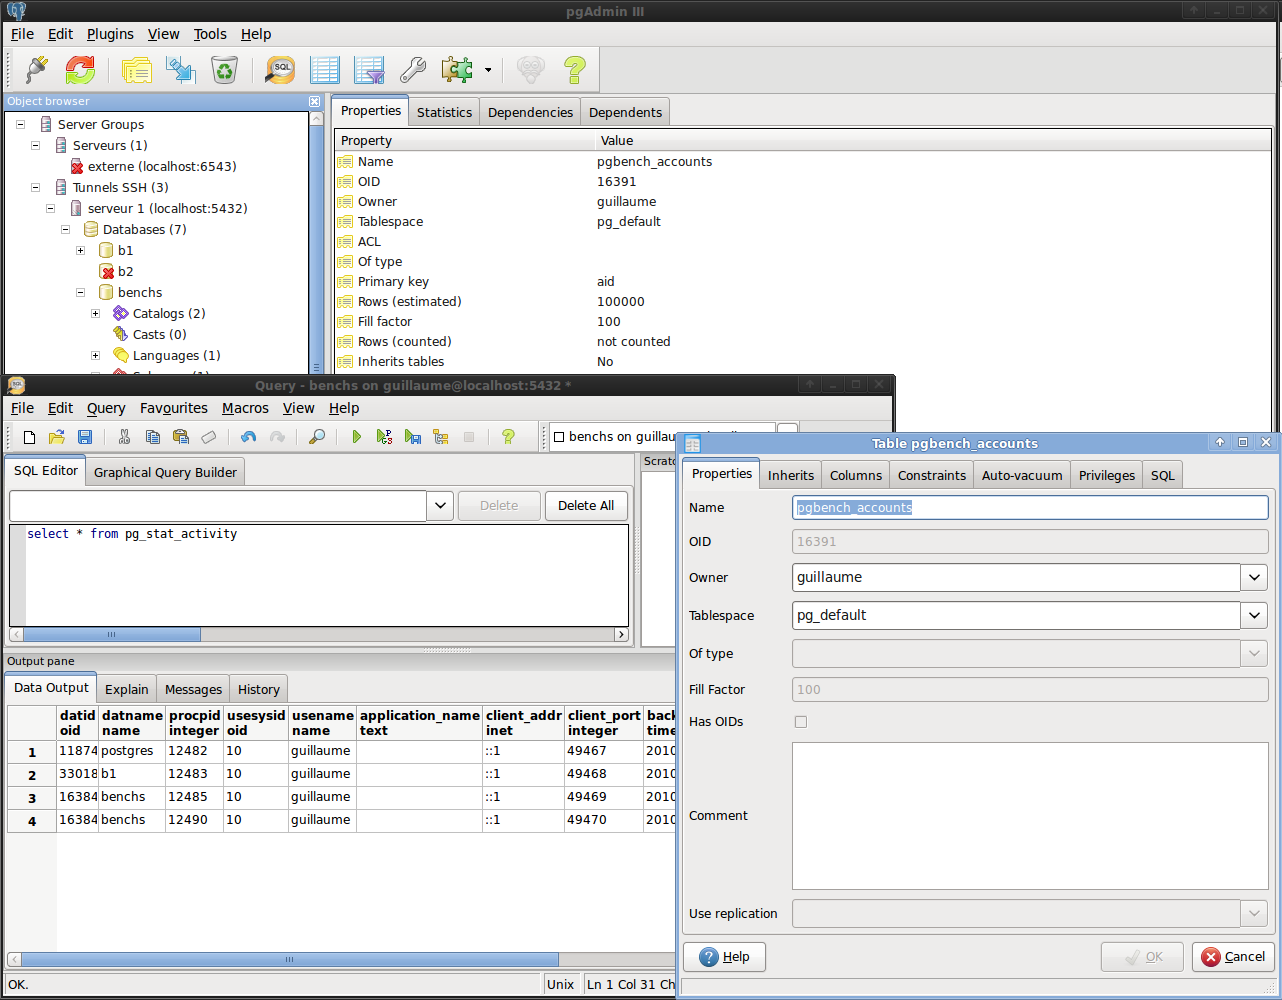
\includegraphics[width=\textwidth]{images/pgadmin3_linux.png}
}

%%%%%%%%%%%%%%%%%%%%%%%%%%%%%%%%%%%
\begin{frame}[fragile]
\frametitle{Creación de tablas}

\begin{block}{CREATE TABLE}
Crea una nueva tabla (vacía) en la base de datos actual y admite un buen número de parámetros (tablas temporales, herencia, valores por defecto, OIDs, restricciones, etc). El usuario que haya creado la tabla será el propietario.
\end{block}

\lstset{caption=Crear tabla ``departamentos'',label=sql:crearTablaDepartamentos}
\begin{SQL}
CREATE TABLE departamentos (
DptoID VARCHAR(10) PRIMARY KEY,
NomDpto VARCHAR(50) NOT NULL);
\end{SQL}
\lstset{caption=Crear tabla ``usos'',label=sql:crearTablaUsos}
\begin{SQL}
CREATE TABLE usos (
CodUso VARCHAR(10) PRIMARY KEY,
DescUso VARCHAR(50),
GrupoUso VARCHAR(20) NOT NULL);
\end{SQL}
\end{frame}

% --------------------------------------------------- Slide --
\begin{frame}[fragile]
\frametitle{Creación de tablas}
%SET DATESTYLE TO 'ISO';
\lstset{caption=Crear tabla ``personas'',label=sql:crearTablaPersonas}
\begin{SQL}
CREATE TABLE Personas (
PersId VARCHAR (20) PRIMARY KEY,
Apellido1 VARCHAR(30) NOT NULL,
Apellido2 VARCHAR(30),
Nombre VARCHAR(30) NOT NULL,
Ciudad VARCHAR (20) NOT NULL,
FechaNac DATE NOT NULL,
HorasExtra SMALLINT DEFAULT 0 NOT NULL);
\end{SQL}
\lstset{caption=Crear tabla ``puestosdetrabajo'',label=sql:crearTablaPuestosdetrabajo}
\begin{SQL}
CREATE TABLE puestodetrabajo (
persid VARCHAR (20) NOT NULL,
estanid VARCHAR (20) NOT NULL,
perfilid VARCHAR (20) NOT NULL,
perfil VARCHAR (50) NOT NULL,
perfilgrupo VARCHAR (20) NOT NULL,
PRIMARY KEY (persid, perfilid));
\end{SQL}

\end{frame}

% --------------------------------------------------- Slide --
\begin{frame}[fragile]
\frametitle{Definir claves externas}

\begin{block}{Mantener la integridad referencial}
Los cambios en una tabla pueden implicar modificaciones en otras tablas relacionadas. PostgreSQL controla esto automáticamente mediante el uso de claves ajenas.
\end{block}

\lstset{caption=Añadir claves ajenas,label=sql:crearForeignKey}
\begin{SQL}
ALTER TABLE estancias 
ADD FOREIGN KEY (coddpto) REFERENCES departamentos(dptoid);

ALTER TABLE estancias 
ADD FOREIGN KEY (coduso) REFERENCES usos(coduso);

ALTER TABLE puestodetrabajo 
ADD FOREIGN KEY (EstanId) REFERENCES estancias(codigo);

ALTER TABLE puestodetrabajo 
ADD FOREIGN KEY (persid) REFERENCES personas(persid);
\end{SQL}


\end{frame}



% --------------------------------------------------- Slide --
\begin{frame}[fragile]
\frametitle{Carga de datos}
\begin{block}{INSERT}
Inserta nuevas filas en una tabla. Se puede insertar una única fila especificada por expresiones de valor, o varias filas, como resultado de una consulta.
\end{block}

\lstset{caption=Insértate en la tabla de Personas,label=sql:insertYourself}
\begin{SQL}
INSERT INTO Personas VALUES('PersId', 'Apellido1', 'Apellido2', 'Nombre', 'Ciudad', 'FechaNac', HorasExtra);
\end{SQL}

Ahora puedes comprobar:
\begin{enumerate}
\item Lo que sucede al introducir un registro con una clave primaria repetida en la misma tabla.
\item Lo que sucede al vulnerar las restricciones especificadas en la creación de las tablas (Ej: Valores nulos o únicos).
\end{enumerate}

\end{frame}


% --------------------------------------------------- Slide --
\begin{frame}[fragile]
\frametitle{Carga de datos masiva}

\begin{block}{COPY}
Utilizaremos este comando para importar y exportar datos entre PostgreSQL y los ficheros del sistema. Este método podrá resultar más práctico y ágil que realizar INSERT.
\end{block}

\lstset{caption=Ejemplo de COPY,label=sql:copy}
\begin{SQL}
-- Para importar datos en ficheros CSV usamos el comando COPY.
-- El comando COPY no es propio del estándar SQL, es específico de PostgreSQL.
COPY departamentos FROM '/home/user/Departamentos.csv' WITH DELIMITER ';' csv header;
-- Ahora importa el resto de ficheros a la base de datos: Usos.csv, Personas.csv y
-- PuestosDeTrabajo.csv
\end{SQL}


\begin{alertblock}{¿Importa el órden?}
Si importas las estancias o los puestos de trabajo antes que las otras tablas te habrá aparecido un error de regla de integridad referencial. No se puede hacer referencia a algo que, por lo que concierne a nuestra base de datos actual, no existe.
\end{alertblock}

\end{frame}


% --------------------------------------------------- Slide --
\begin{frame}[fragile]
\frametitle{Eliminar datos de la DB}

\begin{block}{DELETE}
Este método elimina filas de una tabla que satisfagan la cláusula WHERE o si no hay WHERE, se eliminarán todas las filas de la tabla. El resultado es una tabla válida, pero vacía. Es interesante ver como afecta la existencia de claves ajenas:
\end{block}



\end{frame}


% --------------------------------------------------- Slide --
\begin{frame}[fragile]
\frametitle{Consultas a la BD}

El SQL es un lenguaje estándar de consulta de bases de datos con un gran número de alternativas a la hora de explotar una base de datos. Existen muchos métodos y palabras clave para filtrar, ordenar y combinar los datos. Vamos a practicar un poco:

\lstset{caption=Ejemplos de operadores,label=tab:selects}
\begin{SQL}
SELECT * FROM Personas;
-- SELECT * FROM Personas WHERE Apellido1 = 'tu apellido';
-- SELECT Nombre,Apellido1 FROM Personas WHERE extract(years from age(fechanac)) < 35;
-- SELECT Nombre,Apellido1 FROM Personas WHERE extract(years from age(fechanac)) >= 50 AND extract(years from age(fechanac))<=70;
-- SELECT Nombre,Apellido1 FROM Personas WHERE extract(years from age(fechanac)) BETWEEN 50 AND 70;
-- SELECT NomDpto FROM Departamentos WHERE NomDpto LIKE '%GEO%';
-- SELECT DISCTINCT Perfil FROM PuestoDeTrabajo WHERE Perfil LIKE '%Cate%';
-- SELECT * FROM Personas ORDER BY Apellido1;
-- SELECT Nombre,Apellido1 FROM Personas ORDER BY extract(years from age(fechanac)) asc LIMIT 5 OFFSET 1;

-- Investigad los metodos UNION, INTERSECT y EXCEPT
\end{SQL}

\end{frame}


\end{document}
